% https://www.overleaf.com/6622695572gyrgqvhzstkh

\documentclass{article}

%\documentclass[conference]{IEEEtran}
%\def\BibTeX{{\rm B\kern-.05em{\sc i\kern-.025em b}\kern-.08em
%    T\kern-.1667em\lower.7ex\hbox{E}\kern-.125emX}}
\usepackage{xcolor}    
\usepackage{graphicx} % Allows including images
\usepackage[backend=bibtex,style=verbose-trad2]{biblatex}
\bibliography{bibfile} 


\begin{document}

%%%%%%%%%%%%%%%%%%%%%%%%%%%%%%%%%%%%%%% TITLE %%%%%%%%%%%%%%%%%%%%%%%%%%%%%%%%%%%%%%%%%%%%%%%%%%%
%%\color{blue}

\title{caDDS: Community Assisted Distributed Database for Sequences}

\author{\IEEEauthorblockN{1\textsuperscript{st} Carl Araya}
\IEEEauthorblockA{\textit{Algorithms and Complexity Laboratory } \\
\textit{Philippine Genome Center}\\
\textit{University of the Philippines - Diliman}\\
Quezon City, Philippines \\
jjazcarraga@up.edu.ph}
\and
\IEEEauthorblockN{2\textsuperscript{nd} Cid Azcarraga}
\IEEEauthorblockA{\textit{Algorithms and Complexity Laboratory } \\
\textit{Philippine Genome Center}\\
\textit{University of the Philippines - Diliman}\\
Quezon City, Philippines \\
jjazcarraga@up.edu.ph}
}

\maketitle

%%%%%%%%%%%%%%%%%%%%%%%%%%%%%%%%%%%%%%% INTRODUCTION %%%%%%%%%%%%%%%%%%%%%%%%%%%%%%%%%%%%%%%%%%%%%%%%%%%
% START OF PROGRESS FOR CID MAY 22 2020
\section{Introduction}
The goal of this introduction is to explain the idea of genomes and their size and magnitude. Inside every human body are the instructions to create and maintain it. These instructions are found inside the genome. The the instructions inside the human genome are incredibly long. The entire human genome,inside a singular cell, when laid out is around 2 meters in length. \autocite{ency_sci_tech}

But once all cells are accounted, when all of the DNA of all the cells in the human body are combined. The length can span the earth to moon 6000 times. This describes as well the vast amounts of DNA information in the body. This highlights as well the importance of genomes and genomics. They constitute and contribute important information for all the cells in an organism.


Defining \textit{genome}
% CID PROGRESS ENDS HEREE FOR MAY 22 2020
%------------------------------------------
% CID PROGRESS STARTS HEREE FOR MAY 29 2020

\subsection{Definition of Genomics}
National Institute of Health \autocite{genomics-definition} defines genomics as \\ \\
\textit{Genomics is the study of all of a person's genes (the genome), including interactions of those genes with each other and with the person's environment.} \\ \\


In the definition, one main component of genomics are genes. Genes comprise of DNA. DNA is an acronym that stands for deoxyribonucleic acid. These are more specific information in the cells of organism. DNA is usually denoted by the letters A,T,G,C. These letters symbolize the chemical compounds (or nucleotides) that encode information in the DNA. Another important feature of genes is thar these  are the instructions passed on from one generation to another. \autocite[p.~2]{hartl2018}


These nucleotides form the base pairs (or \textit{bases}). These bases encode information as stated earlier. A clearer picture is that these bases combined act as a blueprint to describe and instruct the body on how to build it and function.\autocite{alberts_mole}

If the bases, genes, genomics combined form the blueprint of the organism. There is a need to understand the complexity and interaction to further understand how an organism works. Genomics play a role in understanding different components of an organism by paying attention to the genes and nucleotide bases. 

The instructions inside the genes describe the complexity which describe an organism. This also means more complex organisms have more complex genes and therefore have a lot more information. Meaning the moment the genomics of complex organisms are studied, more information will be needed and gathered. Humans, being complex, should also have a long set of instructions to detail the complex behaviors. For humans, the full human genome contain around $3.2x10^9$ base pairs \autocite{introgenomics}. This is a lot of information inside the human organism. 

Storing information in the information is one aspect, but before analyzing that information, these have to be taken from the cells and read. Reading these information from genes will need certain technology. The technology is called \textit{Sequencing}.

\subsection{Sequencing}

Reading genetic information found in the DNA uses the technology of Sequencing. The machines are aptly called \textbf{Sequencers} that look (or more appropriately, \textit{read}) the DNA of a specimen. The machine outputs A,G,C,T, sometimes with uncertainties. Sequencers look at the exact order of a single strand of DNA. The process of sequencing DNA seems straightforward that a machine reads only one strand of DNA. In actuality, one strand is too little for one machine to read. So before reading, the DNA is \textit{replicated} multiple times in the laboratory. 

Sequencers also can't read the entire length of DNA. The DNA is also \textit{fragmented} before processing. By fragmented meaning it will be cut up into pieces. These are fragmented since the technology cannot handle reading the entire length of the DNA. Sequencers can only read it in parts. 


The idea of \textit{replication} and \textit{fragmentation} are important because these increase the data taken up when sequencing. Replication causes there are a lot of redundant data when the sequence. Fragmentation causes there to be a need to piece back the information together. Now with those concepts in mind sequencers then reads (or sequences) the replicated and fragmented data.


These reads or sequences taken will need an extra step before the data becomes useful. It will then be needed to be put back together computationally to form the \textit{correct or reference} DNA. These are one of the reasons why genomic data is large because even the fragmented replicated data is still stored, not just the reference DNA.

\subsection{Human Genome Project}

Another way to see the way genomic data is large is by looking at the \textit{Human Genome Project}. The project's aim was to sequence the entire human genome. At the time it needed a lot of collaborations, a lot of financing, and a lot of sequencing, and new computation methods. Back in 2003 was a milestone because the first human genome \autocite{introgenomics} had been first completely read. It took the project ten years of work, a dozen institutions, and 3,000,000,000 dollars to finish. The technology for sequencing and genomics was still at its infancy. 



\subsubsection{Next Generation Sequencing}

%(done) CID: Describe the speedup in terms of what and how the speedup was computed

The introduction of Next Generation Sequencers can be seen as a another significant event in the history of genomics. This is a new technology which has allowed the machines to read faster and cheaper. These utilize a variety of technologies, some make use of light, some use ion semiconductors, others use a special DNA marker with a fluorescent probe \autocite[~p.67]{paulselzer2018}.  


Many countries that research have started employing NGS. Sixteen years later after the HGP, the technology in Japan is very much faster than the technology back in 2003 used for the HGP. The technology in Japan can read 10,000 human genomes per day. \autocite[p.~19]{introgenomics} 

These show how the technology for reading genomes has been developed over the years. This tech has increased the read speed. Which directly affects the speed in which data is produced. Since each read requires storage. This poses a problem to projects involving sequences, the data volumes is usually very large\autocite{bon_compression}. 

There exists a concept of \textit{coverage} as well. Referring back to the \textit{replication} and \textit{fragmentation} concept earlier. There needs to be a specific number of reads a machine needs in order to produce a reference sequence (the correct, standard sequence). Meaning the sequence isn't read only once. 

This contributes to the large data size of sequences. Currently, for a coverage of around 60, the file size for a compressed human genome can easily reach 200 GB. And a project of 10-20 genomes would need approximately 4 TB of storage. Transferring these data across research groups would indeed be a challenge. \autocite[~p.68]{paulselzer2018} These highlight the important and growing problem of storage in genomic research.



\begin{figure}[h]
\caption{Cost per Genome Data Over Time}
\centering
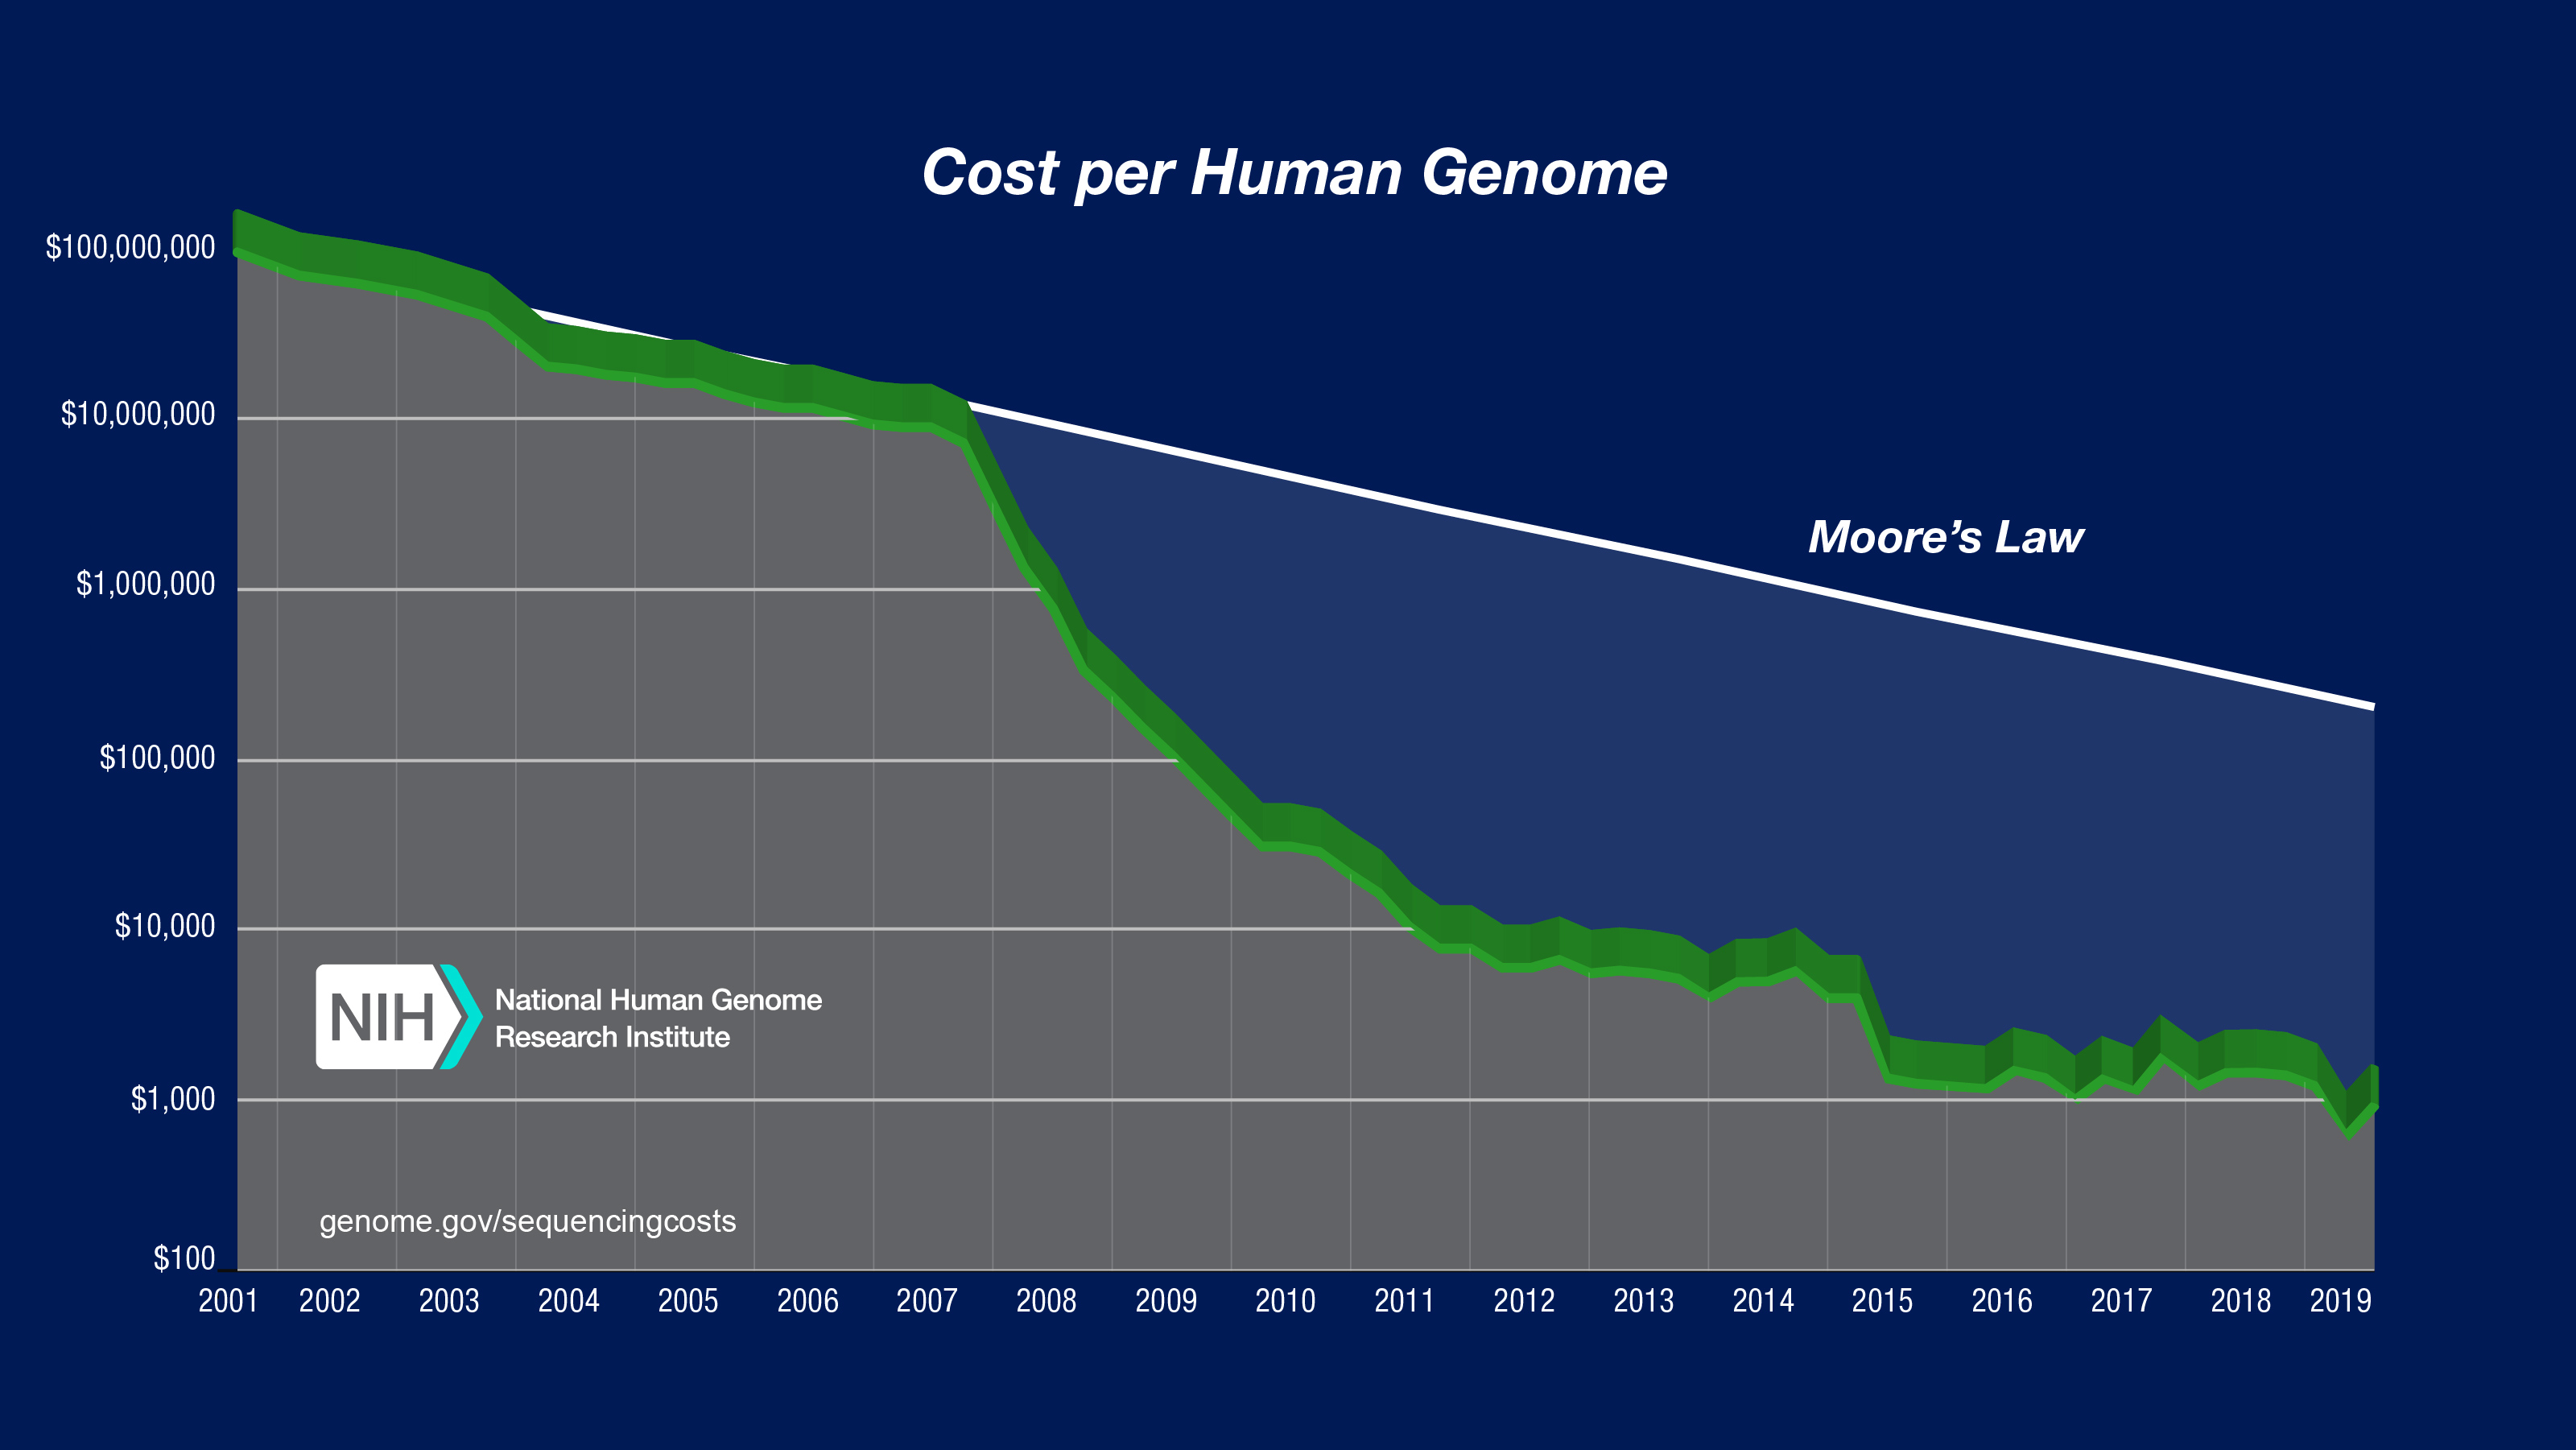
\includegraphics[width=0.65\textwidth]{images/human-gen-cost.jpg} 
\label{fig:human_gen_cost_fig}
\end{figure}

Looking at the Figure~\ref{fig:human_gen_cost_fig} on Page~\pageref{fig:human_gen_cost_fig} \autocite{genomics-cost}, we note the expensive cost at the initial stages of sequencing the human genome. But as time progresses, the cost substantially went down to what it is now. The big fall of the prices around 2004 - 2005 corresponds to the introduction of the Next Generation Sequencers.

\subsection{Database}

\begin{figure}[h]
\caption{Megabase Cost Over Time}
\centering
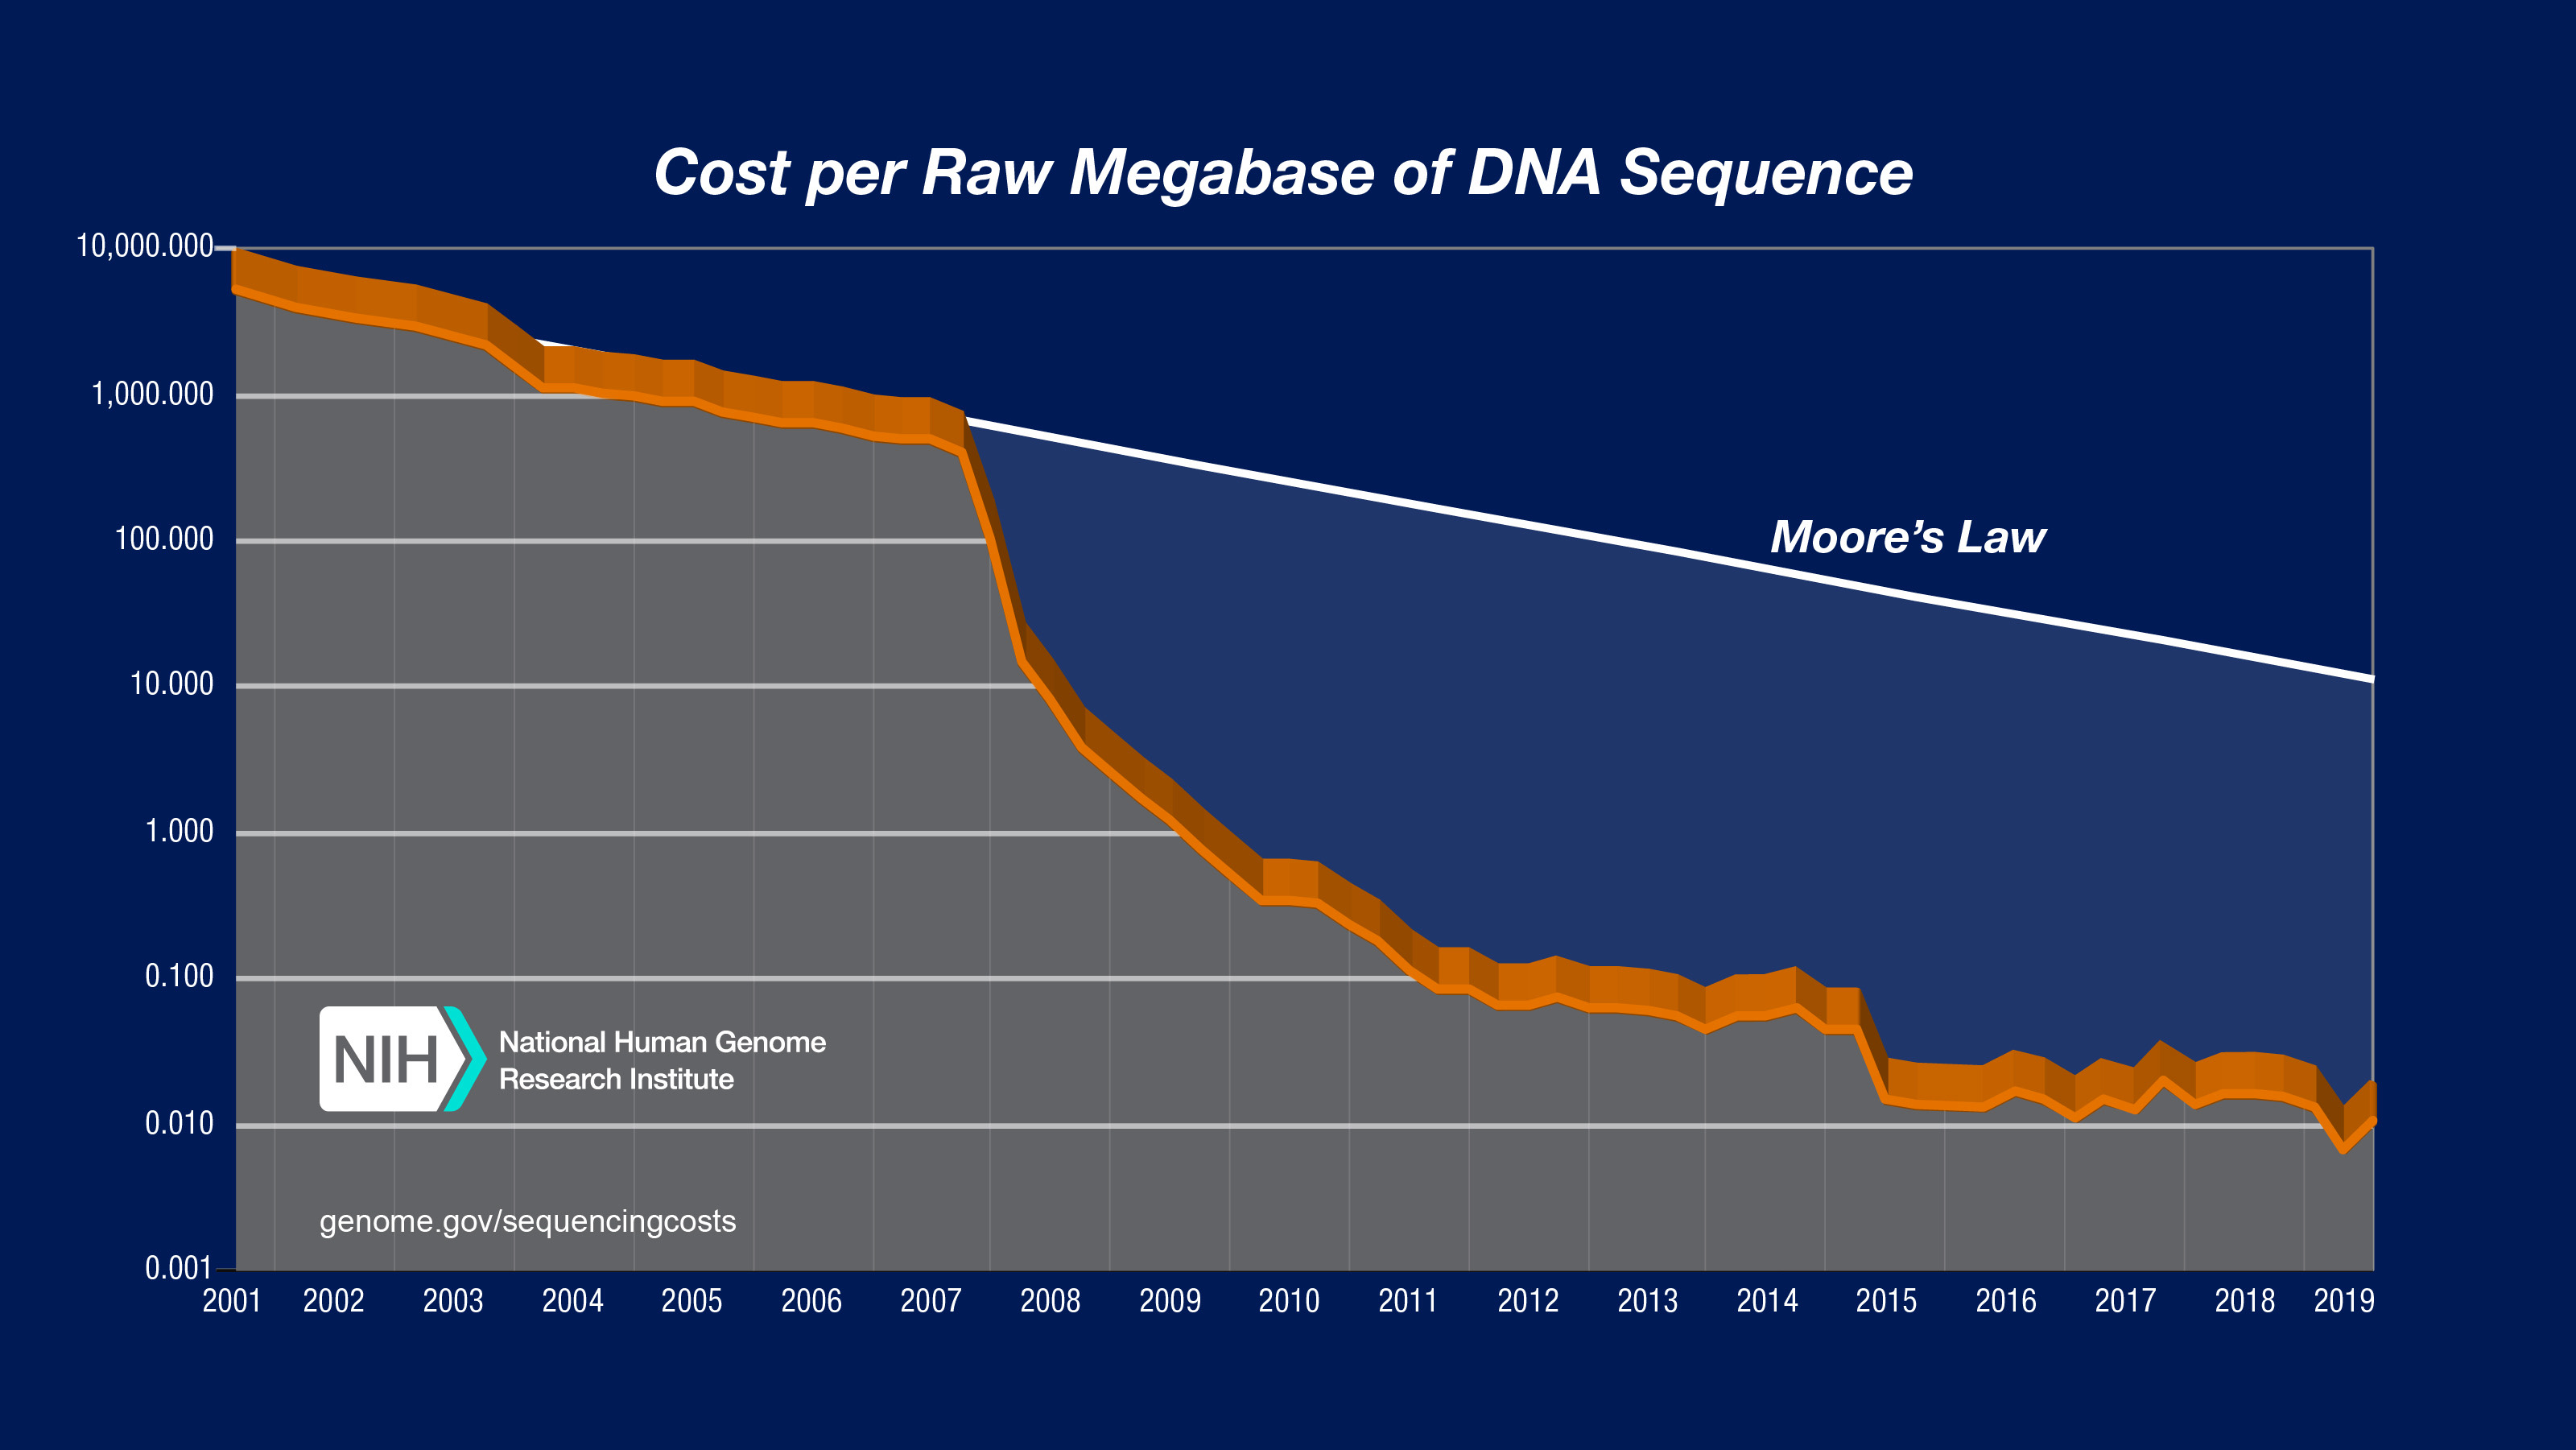
\includegraphics[width=0.65\textwidth]{images/seq-cost.jpeg} 
\label{fig:megabase_cost_fig}
\end{figure}

Similar to Figure~\ref{fig:human_gen_cost_fig} on Page~\pageref{fig:human_gen_cost_fig}, we also note the same pattern for the cost of sequencing (not just humans) in Figure~\ref{fig:megabase_cost_fig}\autocite{genomics-cost}. The cost of sequencing dropped 1000 fold from 2008 to 2012 alone \autocite{bon_compression}. This lowering of cost, makes the idea of sequencing more available. The number of  research projects should also increase as well contributing to the growing number of genomic data.
 
\begin{center}
\textit{Moore's law states that the number of transistors on a chip doubles every two years.}
\end{center}

%CID: An idea: make a quote stating Moore's Law, cite, then explain how this relates to thesis
%KING: Cite and check if true

The idea of Moore's law should give relief to genomic researchers since this means, that as time passes by, technology for processing and storage will improve. And the overall capacity for what technology can do will increase as well. 

But, by paying attention to the speed in which the number of sequence data increases seems to exceed Moore's Law. And this will pose an additional problem since the technology doesn't seem to be catching up. The immediate problem is the storage of all the data being produced. A certain technology needs to be made for the purpose of holding this data. This technology is called \textit{Databases}. But there is a greater need well in making sure the data stays secure, consistent, easily accessible, and fast. These are other aspects needed by a genomic researcher as well. And this is the reason why a specific class of Databases called \textit{Distributed Databases}. Will be needed in this paper.

\subsubsection{Databases Definition}
A database (DBMS, Database Management System) is defined by containing information about a particular enterprise. Functionalities include: \autocite{Silberschatz2010}
\begin{itemize}
    \item Collection of interrelated data
    \item Set of programs to access the data
    \item An environment that is both convenient and efficient to use
\end{itemize}

These form a system that is made for accessing and updating data. The next section discusses the key points when considering how to choose or create a good database system (or DBMS). The key points are important to discuss many important features of the proposed system later. Certain database principles are needed to make sure the data is available, secure, and consistent. 

\subsubsection{Principles of Databases} 
There are 3 principles needed when creating a database. The idea is that only two of the three can be focused on at any given time. Only two since the current technology can only handle two. These principles and limitations need to be taken into consideration when designing the system. \autocite{Silberschatz2010}

\begin{itemize}
    \item Consistency - Does the data have integrity? To update one part, all other (replicated) parts should be updated quickly as well; Data is accurate and copied faithfully. An example would be that genes for specimen A, when copied to another data node should contain the exact copy of the data, with no changes.
    \item Accessibility - How easy it is to access data, API protocols? An example would be the number of commands  a user needs to do to access every data.
    \item Partition Tolerance - How resilient is the system when it comes to failures? If one portion breaks, the other portions should still be entirely usable. An example would be a power failure for one system, how would this affect the other systems?
\end{itemize}

\subsubsection{Database Types} 
Two types of databases will be discussed in this paper. Each have their specific niche and use. One is more efficient and easier to make, another is better suited for collaborative work. Note some technical jargon needs to be used to explain some concepts. These are namely: \autocite{centralizedvsdistributed}

\begin{itemize}
    \item Centralized - In a centralized database, all data are managed by a single DBMS in a single node to be distributed to users. As a result, transactions are easily manageable because everything can be processed in the single node. Here, the cost of communication is high and reliability is low, as an error in the database will mean disaster to the network as a whole. These are easier to create.
    
    \item Distributed - In a distributed database, data are stored in multiple servers in different geographical locations. Each node may contain a part or the entirety of the data. The difficulty of managing transactions will go up, but the result is higher availability, faster response, and modular growth, among other advantages. These databases are better creating spread out databases, and are better for collaborative work.
\end{itemize}

For collaborative genomic work, especially in this paper, distributed databases are most appropriate.

\subsection{Application Architecture}
Another important consideration is how a system is built. These describe the blueprint and interaction within a database system. These provide insights similar to the questions asked when looking between database types. Database types describe how the data is handled inside the system. But application architecture describes how the users interact with the system. The application architecture is how a networked app is structured across the various end systems (i.e. computers, servers, etc.) \autocite{kurose} The end systems are another way to call users or clients. 
The application architecture types fall into either client-server, peer-to-peer, or hybrid architecture.

\subsubsection{Client-Server}
A client-server architecture relies on a Web server that is always
available and has a fixed IP address. When a client (or user) sends a request for data, the server (or DBMS in this example) responds by sending the requested data. The client-server architecture is mainly built to respond to one client at a time. The architecture may handle multiple connections but as these grow bigger, it may not be able to keep up with the increasing number of connections since the server might not be able to handle all the requests.

\subsubsection{P2P}
A peer-to-peer (P2P) architecture has minimal to no reliance on
always-on, dedicated servers. Peers are desktops/laptops (or users) that communicate to each other without passing through a dedicated server (or DBMS). These include internet, BitTorrent, and some other file sharing protocols. An advantage of P2P networks is their scalability, unlike the earlier type. Each user can benefit the whole network by sharing his/her own resources. 

However, since P2P doesn't have a central data management system. P2P has its own problems, which are security and incentivizing users to share their resources.

\subsubsection{Hybrid}
A hybrid architecture combines elements of P2P and client-server architectures, attempting to utilize advantages of both.

For a collaborative genomic system, it would be best to utilize Hybrid Application Architecture. Since there needs to be certain features that Client-Server of P2P might not be able to deliver. One would be scalability, another is security and centralized management of the data.

%%%%%%%%%%%%%%%%%%%%%%%%%%%%%%%%%%%%%%% RRL %%%%%%%%%%%%%%%%%%%%%%%%%%%%%%%%%%%%%%%%%%%%%%%%%%%

\section{Review of Related Literature}

We review the technologies on data storage done before. Some have employed \textit{Client-Server}, some \textit{P2P}, others have tried \textit{Hybrid} (but are still few and unsuccessful).
%CID: Make a transition to go from the diff database types to the explanation of the diff databases

\subsection{SeqTorr: A distributed scalable database for genomic information}
The focus on SeqTorr was finding a way to scale databases meant specifically for genomic information. There was also a focus on being able to choose information to share and use. The standard genomics workflow consists of uploading and downloading data on an international database like NCBI. Having a distributed scalable local infrastructure to store genomic data instead of relying on NCBI would be beneficial since: only certain sequences in NCBI are relevant to the institutions (e.g. Asian sequences are needed more than Caucasian ones), researchers within the country can share data with fast speeds, and  institutions can share in the hosting of data.

The architecture of SeqTorr consists of a master node and multiple data nodes. The master node contains metadata of all the sequences and is where the user authentication is handled, while the data node is where the actual sequences are stored. All user uploads happen in the master node. When the master node receives a sequence from a user, it distributes the sequence to any available data nodes. 
\autocite{seqtorr}

SeqTorr seems to go in the right direction and focus for genomic databses. But currently, SeqTorr is not available, and the code base does not have any documentation which makes future work difficult.



\subsection{BioTorrents}
BioTorrents focused on P2P and making it easy to share data across biological scientific communities.  Scientific data continues to grow, and so does the demand for easier accessibility. Centralized servers, as stated earlier, using HTTP or FTP cannot keep up with concurrent requests, and peer-to-peer protocols does not scale well for large files.\autocite{biotorrents} One example of these centralized servers is NCBI, which will be discussed later. BitTorrent handles both these problems. 

BioTorrents is a system for legally sharing scientific data that works on top of the BitTorrent protocol (or P2P). It is much like a public tracker. The main website hosts .torrent and metadata files. The main website doesn't store data, rather it lets the users keep the data and share it to other users. The main website only facilitates the sharing of these data (via the idea of P2P and torrents).

The main website stores info about each dataset includes categories, license, filenames, etc. that helps users in searching for relevant datasets. There is also a torrent file has a list of trackers, servers that "know" which peers are serving which files, so it can download from those peers simultaneously. These torrents act like a directory telling the user who currently has the data for a piece of the file. The system then helps the user download many pieces of the file from many different users.

The client (or user) must have their computer continuously turned on to keep their file available to others. The main issue with BioTorrents, which is a problem as well in P2P, is that it requires lots of users that will keep many torrents available as often as possible.\autocite{biotorrents} These entail that for the system to work, many people need to use it and all these people need to keep their computers on all the time.

BioTorrents was successful, many people had used it to share data. It was active for a while. However, BioTorrents has been down for years. This also shows what problems a system will face when doing a pure P2P application architecture.

\subsection{PeerDB}
% summarize intro
PeerDB is a proposed P2P system for sharing general data. Each node is equipped with a MySQL database that it keeps available for other nodes to download from. Each node also keeps track of its neighbors, and any useful information about them. Queries are passed around neighbors, with a maximum number of hops. A node may cache information about other peers to speed up future queries.
\autocite{peerdb}

PeerDB is a proposal for a distributed system using P2P. For this to be used in the context of genomic biological work, a main website which facilitates sharing will be need to be put up. PeerDB needs to be installed as well on all the users who will be participating.

A future PeerDB system will also face similar problems faced by BioTorrents since it will need to rely on numerous active users for it to work.

\subsection{NCBI}
NCBI was discussed briefly in the section on \textit{BioTorrents}. It uses a client-server architecture. Users may download data via the graphics interface (website), or may be done via FTP or HTTP \autocite{biotorrents}. The latter is preferred since it may be done to automate the download of data.

The SeqTorr authors\autocite{seqtorr} stated that NCBI is the main and current DBMS used to get and share genomic data. But one difficulty using that is updating the current genomic data. There currently is no way to check which data (on your computer) has been updated, which sequences were corrected. And the way the authors solved this was to regularly re-download the entire NCBI database.

To state again some problems of NCBI, it has the limitations of \textit{Client-Server} architecture meaning the speed of the download is heavily reliant on the speed of the main NCBI server. Which also puts a lot of stress on the main server. Another problem discussed earlier was the updating of data, which have no technology yet to do so.

% CID PROGRESS ENDS HEREE FOR MAY 29 2020
% CID PROGRESS STARTS HEREE FOR JUNE 2 2020

\begin{table}[h]
    \caption{Comparisons of Different Databases}
    \begin{tabular}{|l|l|l|l|l|}
    \hline
    System      & CS/P2P/H & Available? & DL/UL speed & Type of Data \\ \hline
    BioTorrents & P2P           & No         & Depends                    & Biological  \\ \hline
    SeqTorr     & H             & No         & Fast (PH server)           & FASTA        \\ \hline
    PeerDB      & P2P           & No         & Depends                    & General      \\ \hline
    NCBI        & CS            & Yes        & Slow (US server)           & Biological  \\ \hline
    \end{tabular}
    \label{table:database_comparison_table}
\end{table} 

Table~\ref{table:database_comparison_table} on page ~\pageref{table:database_comparison_table} describes the different technologies done. This will also be used to decide what are the main problems of the different databases.


\section{Problem}
To restate the different gaps or problems found with other implementations
\subsection{Problems of Classical Databases}
\begin{enumerate}
\item Genome researchers download an entire database of genomic data, especially when uncertain how to update their data
\item Genome researchers only need a portion of the database, but end up downloading the entire database
\item Client-Server approach can face bottlenecks (server speed)
\item P2P approach has a need of a large unmoderated active user base to work

\end{enumerate}

\subsection{Problems of Distributed Databases}
\begin{enumerate}
    \item No existing public usable framework on distributed database for genomes
    \item Existing distributed database for genome code has no documentation
\end{enumerate}

\section{Objectives}


Based on the problems we found earlier, we propose to:

\begin{itemize}
    \item Design the framework for an information system that speeds up the download and upload of genomic data
    \begin{itemize}
        \item To resolve 1 \& 2 of the Problems of Classical Databases. 
    \end{itemize}
\end{itemize}

\begin{itemize}
    \item The system should have the main API’s
    \begin{itemize}
        \item POST genome data
        \item GET genome data (implement hybrid P2P)
        \begin{itemize}
            \item This will aim to resolve and speed up number 3 in the Problems of Classical Databases
        \end{itemize}
        \item PUT genome metadata (optional: PUT data)
        \item DELETE genome data
    \end{itemize}
    \item Write a documentation for the system
    \begin{itemize}
        \item This will be used to resolve the Problems of Distributed Databases
    \end{itemize}
\end{itemize}

%KING: Use Genomic Data instead of genome data



\section{Scope}
%(done) CID: pahabain pa konti

The project will focus mainly on the functionalities of the system, and not focus much yet on the different possible data types and data in the system. Therefore the current scope and coverage of the project:

%(done) KING: This sentence does not make sense (the coverage is only: security and authenticaion is not part of the scope), make it sound that it will work when it isnt in bullet form
%(done) CID: Weird sentence, just rephrase

\begin{itemize}
    \item will be the use of only the FASTA file format
    \item will be the use of only the DNA nucleotides
    \item will only a proof of concept, UI will be purely for functional purposes
(very basic design)
\end{itemize}

The current scope and coverage of the project will NOT contain:

\begin{itemize}
    \item Security and Authentication
\end{itemize}

Inside the university there are many problems associated with having security when using network resources, that is why authentication will not be part of the scope.

\section{Theoretical Framework}

\subsection{Networks}

%KING: everyone is assumed to know networks
%(done) KING: Please cite
%CID: Can reduce the discussion here. Then emphasize the importants parts
Networks Layers are the abstraction of how computers pass data to each other. This is needed to maximize the speed in which data is transferred between computers. A network, specifically the Internet, is comprised of the following levels of abstraction. \autocite{kurose}
\begin{enumerate}
    \item Level 1: Medium used to send signals (physical, electrical signals of 0
and 1), through wire or by air
    \item Level 2: Introduction of packets: Wifi, Ethernet, connecting together
different . Goal of sending a group of signals.
    \item Level 3: Introduction of networks: IP Address to uniquely identify
entities.
    \item Level 4: Management of error free data transmission: Sending a group
of messages via TCP, UDP, FTP
    \item Level 5: Abstraction of Level 4: Function calls programmers will use
to do level 4 processes.
\end{enumerate}

Level 1 through 3 focus on building a system for sending messages from one computer entity to another. And this isn't important for the thesis, but important to understanding the scope of what the thesis will do.

Level 4 and 5 here is where this thesis will dwell upon. Since this is more specific to what the thesis will be needing, such as file transfer, checking if the files are error free, and more.
%CID: expound this sentence more


% (partially done) CID: Explain POST PUT GET DELETE in relation to CRUD, idk if needed to

In networks, when there is data being accessed over the network, it is not called C.R.U.D., instead it is called POST, GET, PUT, DELETE. POST is analogous to CREATE meaning the user submit data to be stored (in the server). GET is similar to READ but is in the context of reading a file over a network (from a server). PUT is analogous to UPDATE as DELETE remains as DELETE. These are codes used to denote network commands that do the same thing as the CRUD functions discussed earlier. This is important since there is an added layer of difficulty when it comes to transmitting data over a network.

%(partially done) CID: Have a paragraph summarizing what the system does (Like expanded version ng objectives pero mas may technical shizz)

\subsection{Summary of the System}
The system is essentially a database. The database stores sequence data. It has the normal CRUD functions meaning Create, Read, Update, Delete. It can let anyone download sequence data. But only registered users can upload sequence data. When a user uploads data, the moderator will verify the data's authenticity before allowing it to be uploaded. Then for the downloading the data. The user will experience a normal download, but under the hood the system will be doing a lot of work. It will check multiple "mirrors" of the download, by looking at the different available data nodes, then let the user choose the fastest or best option. File transfer will occur, then the system will be the one checking if the file were downloaded correctly. There is a simple organization of available files as well.

%(partially done) CID: the paragraph above is still informal

%(done) CID: Also explain why title is that

The system is described as \textit{community assisted}. Since ideally, institutions can contribute to sharing the data by hosting servers that will become the data nodes. This sharing allows a greater bandwidth, and hopefully speed in which this data can be transferred. The speed will be measured in order to measure if this project achieved its objective. The database is a distributed database, which will aim to utilize the best features from Peer2Peer and Client/Servers. This will also aim to store sequences. Thus the "Distributed Database for Sequences" portion of the title.

\begin{figure}[h]
\caption{App network diagram}
\centering
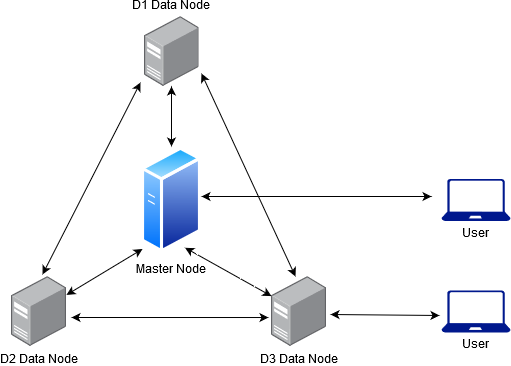
\includegraphics[width=0.35\textwidth]{images/thesis1.png} 
\end{figure}

%CID: Explain briefly each figure

\begin{figure}[h]
\caption{POST: Uploading a sequence to the master node}
\centering
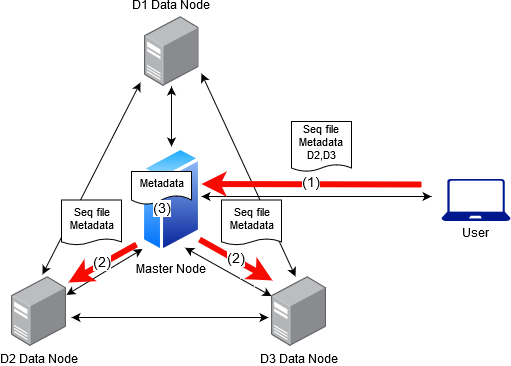
\includegraphics[width=0.35\textwidth]{images/thesis3.png} 
\end{figure}

\begin{figure}[h]
\caption{POST: Uploading a sequence to the data node}
\centering
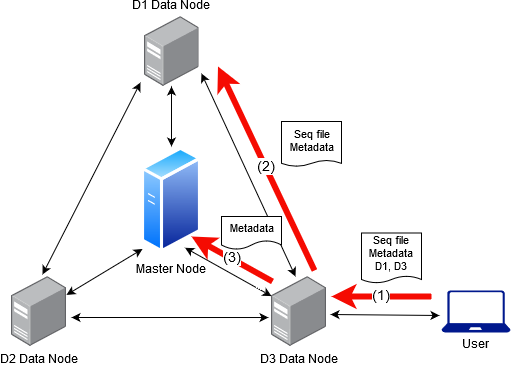
\includegraphics[width=0.35\textwidth]{images/thesis2.png} 
\end{figure}

\begin{figure}[h]
\caption{GET: Downloading a sequence}
\centering
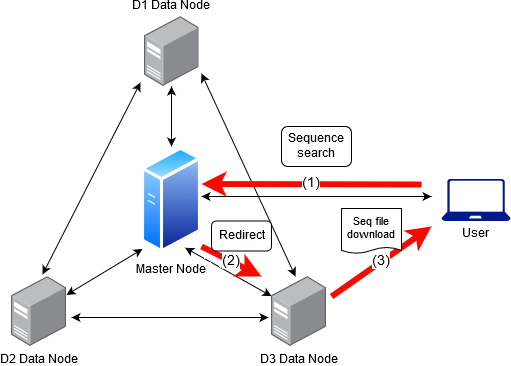
\includegraphics[width=0.35\textwidth]{images/thesis4.png} 
\end{figure}

%CID: Explain the data model and data permissions

%CID: Data Model, make sure to cite this in a paragraph

\begin{table}[h]
\caption{Data Model to be Used in the System}

\begin{tabular}{c|c}
\hline
    key & description \\
\hline
\hline
    seq\textunderscore id & unique ID assigned to all sequences \\
    organism & organism where the sequence was extracted from \\
    quality & the rating of the data based on the number of downloads or another criteria \\
    uploader & user that uploaded the data \\
    institute & institute where the uploader or sequence was taken from \\
    upload\textunderscore date & date the data was uploaded to the database \\
    last\textunderscore modified & the date the metadata or data was edited \\
    data\textunderscore nodes & list of data nodes that this data is contained to
    

\end{tabular}
\label{table:data_model_table}

\end{table}

Table~\ref{table:data_model_table} on Page~\pageref{table:data_model_table} aims to show the metadata that will be initially stored in the database.

%CID: Data Permissions

\begin{table}[h]
\caption{Data Permissions and Users in the System}
\begin{tabular}{c|c}
\hline
    user & description \\
\hline
\hline
   Moderator & Has ability to upload, download, store data, verify \\
    Peer & Has ability to upload, download, store data \\
    Guest & Has ability to upload, download \\
    

    
\end{tabular}
\label{table:data_perm_table}
\end{table}

Table~\ref{table:data_perm_table} on Page~\pageref{table:data_perm_table} shows the different set of users and the permissions allowed to them in the system. The moderator is a special user who has the ability to not allow some data to be uploaded. This is to make sure there is a means to verifying the data being uploaded. All users can upload, download, and store (or host) data. All other users, which are called guests has an ability to download and upload data.


\section{Proposed Methodology}

% CID: explain the 3 main phases (system creation, testing, documentation)
% CID: explain the importance of each phase
% CID: explain

\subsection{Creating the system}
The system will be needed to be done before any of the following steps can occur. 
\begin{enumerate}
    \item Set-up database architecture
    \item Code the POST API
    \item Code the DELETE API
    \item Code the PUT API
    \item Code the GET API
    \begin{enumerate}
        \item As a classic database
        \item Revise to have distributed database functionality (may be moved to item 1) 
        \begin{enumerate}
            \item Code data node
            \item Deploy \& test functionality of data node/s
            \item Code master node
            \item Deploy \& test functionality of master node/s
            \item Test interoperability of nodes
        \end{enumerate}
    \end{enumerate}
\end{enumerate}

\subsection{Testing}
Part of the goal of the project is to implement a better data transfer mechanism. And one way to verify this is to see the speed in which the system compares to other systems.

\begin{enumerate}
    \item Create test for testing original speed
    \item Test original download speeds
    \item Create test for testing new speed
    \item Test new speeds
\end{enumerate}


\subsection{Documentation}
Another part of this project's goal as well is to make this available and usable for the community. And documentation will help make the system easy to use, manage, and develop.
\begin{enumerate}
    \item Compiled to a PDF that is easy to read
    \item How to use (all users)
    \item How to set up
    \item How to maintain and add features
\end{enumerate}

\subsection{Resources needed}

Servers must have networking capability and at the very least have their HTTP port configured to be open to each other, or optionally, the HTTP port can be open to the Internet.
\begin{enumerate}
    \item 1-2 servers in PGC to serve as master node (1 minimum; the other server will serve as data node)
    \item 1-2 servers in DCS to serve as data nodes (1 minimum)
    \item 2 workstations where both of us can program the system
    \end{enumerate}

\printbibliography

\end{document}